\subsection{Parametrisierung}
Während der Tests ist stark aufgefallen, dass das Regressionsverfahren sehr parameterabhängig ist. Wie im vorherigen Kapitel zu sehen ist, liefert die implementierte Lösung mit der richtigen Parametrisierung ein gutes Verhalten. 
Bei falscher Parametrisierung wird die Verfolgung sehr viel schlechter bis unmöglich.\\
Große Unterschiede gibt es bei geraden und kurvigen Objekten. Als ausschlaggebende Parameter stellten sich die Gewichtungen der einzelnen Fehlerarten, die stärke \textit{Tikhonov Regularisierung} (siehe Gleichung \ref{F-function}) und der maximale Gesamtfehler der Regression bis zu einer Transformation (siehe Abschnitt \ref{alterWorldCoords}) heraus.
Bei geraden Objekten führt eine Gleichgewichtung der Fehlerarten, eine starke \textit{Tikhonov Regularisierung} und ein hoher erlaubter Maximalfehler zu sehr guten Ergebnissen (vgl. \ref{sec_pendel}).\\
Kurvige Objekte, wie in Abb. \ref{testSCurve} oder \ref{testStraightCirc} führen am besten bei einer höheren Gewichtung des Orientierungsfehlers, keine \textit{Tikhonov Regularisierung} und ein geringerer erlaubter Maximalfehler zu guten Ergebnissen.
Problematisch ist, dass die \textit{falsche} Parametrisierung (z.B. hoher Maximalfehler für kurvige Objekte) im schlimmsten Fall zu einem großen Fehler, damit einhergehendem Sichtverlust zum Objekt und einem schlecht geschätzten Polynom führt, dass keine erneute Annäherung zum Objekt mehr gelingt.\todo{hier fehlgeschlagene tests}

\subsubsection{Einpendeln}
\label{sec_pendel}
In jedem Testlauf fiel auf, dass bei erster Sicht des Objektes eine Art \texttt{Einpendeln} stattfindet, also ein zuerst großer Fehler, der dann über mehrere Meter beständig abnimmt, bis eine stabile Fahrt über dem Objekt erreicht wird. Diese Beobachtung konnte auch beim Wechsel von geraden Objektverläufen auf kurvige Verläufe gemacht werden.\\
In Abbildung \ref{figpendel} ist diese Beobachtung mit verschiedenen Parametrisierungen dargestellt.

\begin{figure}[H]
\begin{tabular}{cc}
\subfloat[Sehr gute Parametrisierung mit Gleichgewichtung der Fehlerarten, \textit{Tikhonov Regularisierung} und hohem Maximalfehler.]{\includegraphics[width=0.5\textwidth,height=0.3\textheight]{/testlaeufe/gradeGut/groundTruthPosition.jpg}}&
\subfloat[Gute Parametrisierung mit Gleichgewichtung der Fehlerarten, geringer \textit{Tikhonov Regularisierung} und weder hohem, noch geringen Maximalfehler.]{\includegraphics[width=0.5\textwidth,height=0.3\textheight]{/testlaeufe/Gradeok/groundTruthPosition.jpg}}\\
\subfloat[Schlechte Parametrisierung mit höherer Gewichtung des Orientierungsfehlers, keiner \textit{Tikhonov Regularisierung} und geringen Maximalfehler.]{\includegraphics[width=0.5\textwidth,height=0.3\textheight]{/testlaeufe/Gradeschlecht/groundTruthPosition.jpg}}
\end{tabular}
\caption{Testlauf mit einem geraden Objekt [Abb. \ref{testStraight}] mit unterschiedlicher Parametrisierung. Im Fehler der AUV-Position zur Objektposition ist zu erkennen, dass bei den guten Parametrisierungen der Fehler über die Zeit abfällt. Bei der sehr guten Parametrisierung (\textit{a)}) sogar noch weitaus schneller. Bei der schlechten Parametrisierung (\textit{c)}) findet keine Verringerung des Fehlers statt. Die Höhe der Ausschläge nehmen auch nicht beständig ab, wie bei den guten Parametern.}
\label{figpendel}
\end{figure}

\subsection{Systematischer Fehler}
\label{sec_sysError}
Während einiger Testläufe gab es längere Bereiche, in denen stets mit einem leichten Versatz zum Objekt gefahren wurde. Sehr deutlich zu sehen ist dieses Verhalten in den Abbildungen \ref{fig_leftCurve}, \ref{fig_rightCurve} und \ref{testSCurve}. Betrachtet man bei diesen drei Abbildungen jeweils den Fehler der detektierten Objektposition zur realen Objektposition fällt auf, dass der Fehler um einen bestimmten Wert verteilt ist und einen systematischen Fehler andeutet.\\
Für das Auftreten dieses Fehlers gibt es einige mögliche Erklärungen.
Zum einen fällt auf, dass der systematische Fehler meist nach scharfen Kurven oder teilweiser Unsichtbarkeit des Objektes auftreten. Da die implementierte Lösung bei ausbleibenden Ergebnissen der Objekterkennung die Fahrthöhe erhöht, um den Sichtbereich zu vergrößern und bei erneuter Sichtung wieder auf die Zielhöhe korrigiert, wird nach einem Bereich ohne Detektion stets abwärts gefahren, was zu einem erhöhten Pitch-Wert führt.\\
Bei scharfen Kurven wird durch die Fahrteigenschaften ein höherer Roll-Wert erreicht, als bei gerade Fahrt.
Der systematische Fehler tritt also oft direkt nach Situationen auf, die eine unruhige Fahrt verursachen können. Dies lässt darauf schließen, dass die Transformation von 2D- in 3D-Koordinaten (vgl. \ref{section_PicToCam})für den Fehler verantwortlich ist.\\
Eine andere mögliche Erklärung ist darin zu finden, dass das Objekt in den Bereichen mit systematischen Fehler oft leicht verdeckt ist. Verdeckte Objekte führen dazu, dass das Objekt im Binärbild schmaler erscheint. Da die Detektion im Binärbild über eine Box mit der erwarteten Breite des Objektes im Bild durchgeführt wird, führt ein schmaler erscheinendes Objekt zu Problemen. Bei optimal sichtbaren Objekten \textit{passt} diese Box am besten (die meisten Inlier), wenn der Mittelpunkt der Box in horizontaler Richtung genau in der Mitte des Objektes liegt. Bei schmaler erscheinenden Objekten \textit{passt} die Box auch an weiteren Stellen des Objekten genau so gut, wie in der Mitte. Durch den Zufallsaspekt des \rans -Algorithmus kann hier ein breiter Bereich als Objektmitte detektiert werden.\\
Gestützt wird diese Möglichkeit auch durch die Tatsache, dass die Streuung des Fehlers in Bereichen mit systematischen Fehler weitaus größer ist.
\todo{hier grafik}
Eine dritte Möglichkeit ist ein Fehler in der Odometrie des Fahrzeuges. Bei leichten Fehlern in der Positionsschätzung wird durch die Transformation von Body- in Weltkoordinaten dieser Fehler auf die detektierte Objektposition übertragen.
\todo{Max kann das sein? Kann man das irgendwie Prüfen?}